\section{Evaluation of WhiteMesh Channel Assignment}
\label{sec:experimentdesign}

% Adjust the order of the results and explain the result more in detail

We now extensively evaluate our proposed measurement-driven heuristic 
algorithm against the upper bound approaching formed by our integer 
linear program and versus prior channel assignment strategies. We 
introduce the topologies and metric calculation used in the analysis 
and present a set of results based on the linear program and heuristic algorithm.

\subsection{Experimental Evaluation Setup}
\label{subsec:design}
% Simulation Setup
A key aspect of WhiteMesh networks is the diversity in propagation from the lowest white
space channels (tens to hundreds of MHz) to the highest WiFi channels (multiple GHz). Thus, 
to evaluate the performance of our measurement-driven algorithm, we consider a wide range 
of propagation characteristics from four different frequency bands.  For white space bands, 
we choose 450 and 800 MHz, for WiFi bands, we choose 2.4 and 5.8 GHz according to the measurements
from~\cite{pcuiwinmee}. 
In the 9 measurements from~\cite{pcuiwinmee}, we map the population density from US 
census~\cite{uscensus} to the activity level for each bands as Table.~\ref{tab:activitymeasurement}.
The measurements connect the relation of population distribution, traffic demand,
and available channel capacity in multiple bands. 
We input the measurements to the ILP and heuristic algorithm to calculate
the available channel capacity $\delta$ for our algorithm which makes the available channel 
capacity of all the bands more practical. With the same transmission
power and antenna gain, the highest carrier frequency would have the shortest communication range.
Hence, we set a communication-range threshold of -100 dBm, and normalize the communication 
range with the highest frequency of 5.8 GHz. In particular, the communication range of 
450 MHz, 800 MHz, 2.4 GHz, and 5.8 GHz would be normalized to 12.8, 6.2, 2.4, and 1, respectively 
according to Eq.~\ref{eq:friis}. The interference range is computed as twice that of the communication 
range~\cite{raniwala2005architecture}. We deploy static wireless mesh networks of $n$ 
mesh nodes along a regular grid with a normalized distance of 0.8 between rectangular edges. 
The gateways are chosen through a typical cell hexagon deployment method based on 2.4 GHz~\cite{meguerdichian2001exposure}.
Unless otherwise, specified in the analysis, all four bands are used in the WhiteMesh
topology studied. For practical application scenarios, more channels could be involved in the 
algorithms.


The throughput achieved through the gateways is not only critical for network vendors (e.g., cellular
carriers charge fees for total bandwidth through towers), but also has been used by researchers
to evaluate channel assignment~\cite{avallone2008channel}.  As mentioned previously, the wireless
capacity of gateway nodes has been shown to be the bottleneck in mesh networks~\cite{robinson2010deploying}.
Moreover, traffic arrived gateway is affected by multiple factors, such as mesh node placement, gateway placement, 
routing, and channel assignment, the latter of which is the focus of our analysis and algorithms. 
For the purposes of our analysis, we specifically calculate the traffic arrived gateway first introduced
in Section~\ref{subsec:problem} in the following way.  Mesh nodes that have a close hop count path to the gateway
nodes are the first ones served. Where there are nodes with the same hop count, the least interfering
mesh nodes are chosen for serving. Then, the demand of multihop mesh nodes are served 
until there is no remaining demand to be satisfied or there is no remaining channel capacity through any path.

% NEWClaim fix, map mesh node offer load to population distribution configurateion
Through the algorithms, we investigate the impacts of network size, bands availability, and channel occupancy
on wireless white mesh networks. We vary the average population distribution and the available channel 
capacity according to~\cite{pcuiwinmee} of the target area, assuming 10\% of the residents will use
our service. An individual would have a 100 KB/s traffic demand on average. Then, we assign the demand 
to users randomly under the same average value across the area and run the analysis of each case 20 times 
as the simulation configuration. Through the assignment, the traffic arrived at gateway nodes and the 
network throughput are calculated. To approach the traffic arrived gateway up-bound, we relax our ILP 
model to keep the link capacity constraints, given the demand of the mesh nodes as a parameter to 
achieve the maximum throughput at the gateways. 
We compare BPS with the 
{\it (i)} Common Channel Assignment (CCA) from~\cite{draves2004routing},
{\it (ii)} Breath First Search Channel Assignment (BFS-CA) from~\cite{tang2005interference}
under the same configuration.
In typical CCA~\cite{draves2004routing} algorithm, two nodes will assign a common channel 
for each other when both of them share free radios working in the same channel. 
In BFS-CA~\cite{tang2005interference} algorithm, a node will search all the 
available one-hop connections then choose the one has the largest available capacity for a new assignment. 
These two methods focus on multi-channel assuming the existing links are equal 
when there is no assignment on the channel. In BPS, we both consider and 
leverage propagation differences of diverse bands.
The ILP Bound calculation make the mesh nodes activate all possible connection 
the gateways if there exists a path. However, the three heuristic algorithms 
provide assignment each mesh node has connection only to one gateway in the network, and this reduce 
the dynamic changes for the assignment, which could be implemented by updating the assignment in a 
short term through the heuristic algorithms.

\subsection{Experimental Analysis of WhiteMesh Backhaul}
\label{subsec:analysis}

\subsubsection{Network Size \& Bands Effect}

%\begin{figure}
%\vspace{-0.0in}
%\centering
%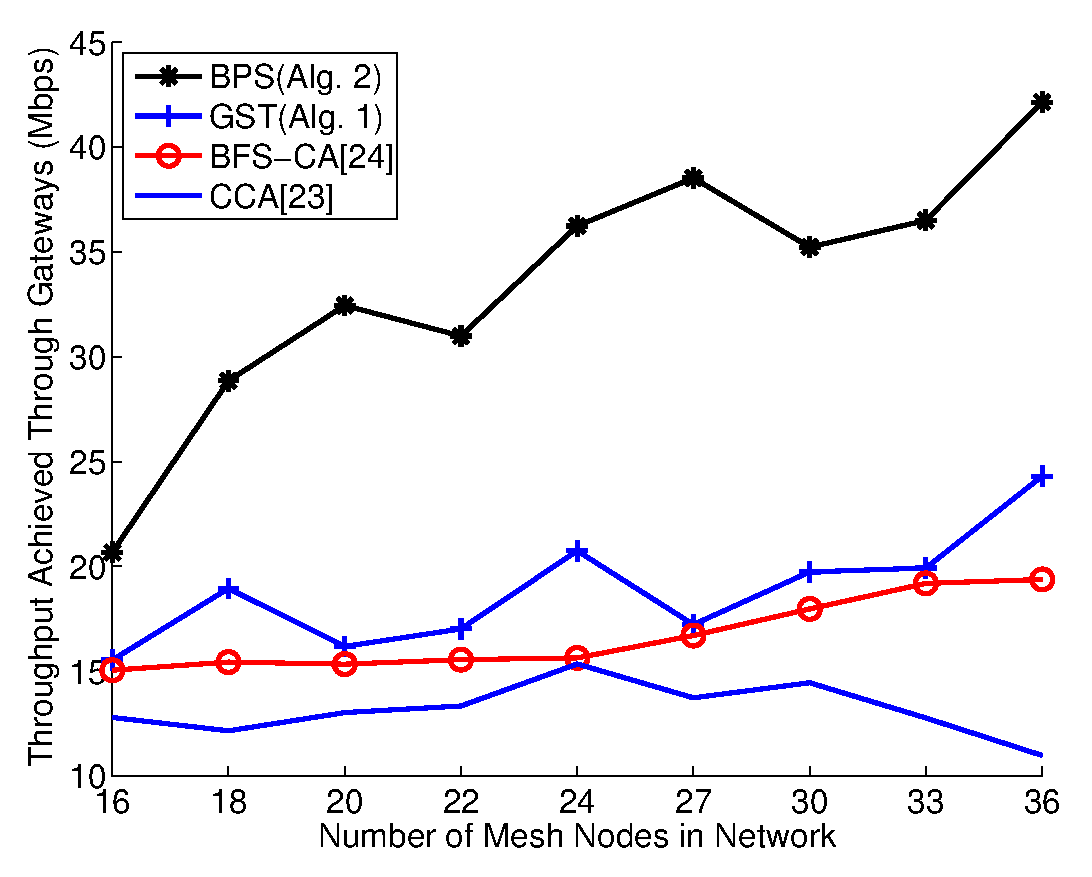
\includegraphics[width=84mm]{figures/varysize}
%\vspace{-0.1in}
%\caption{Average Population Distribution = 500 $ppl/km^2$}
%\label{fig:varysize}
%\vspace{-0.2in}
%\end{figure}
%
%
%\begin{figure}
%\vspace{-0.0in}
%\centering
%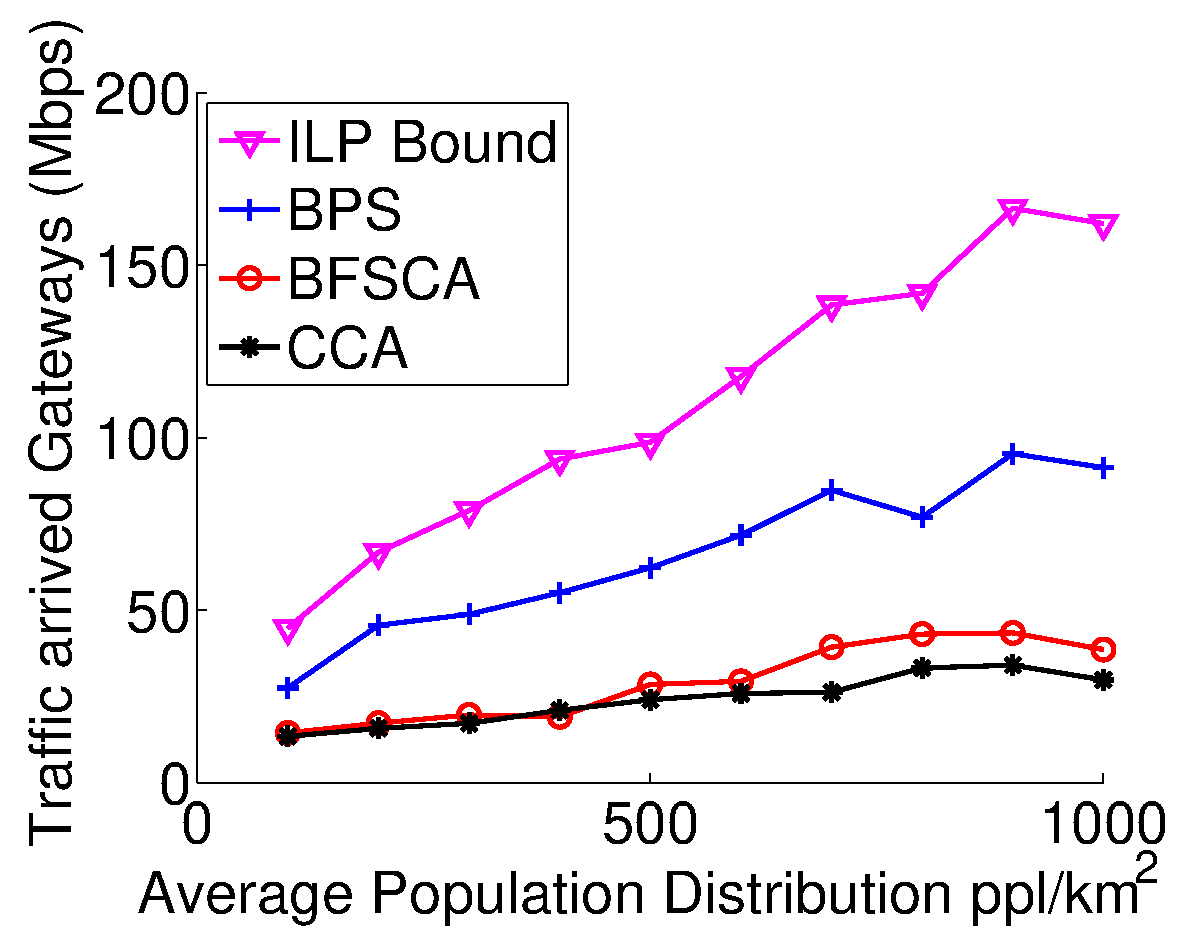
\includegraphics[width=84mm]{figures/maxtpt}
%\vspace{-0.1in}
%\caption{Varying Load, 49-Nodes Regular Grid}
%\label{fig:maxtpt}
%\vspace{-0.2in}
%\end{figure}



% Meat chapter

% ILP bound
Typically, clients and mesh nodes have diverse traffic patterns with
the download direction dominating the total traffic demand (e.g., consider
service agreements for cellular data or Internet connectivity). Hence, to
simplify the analysis and scale the ILP Bound to larger network sizes, we 
only consider the download traffic while maintaining the simulations.
We then assign distributed download traffic demand randomly per 
mesh node with a maximum offered load to simulate the practical scenario 
as specified in Fig.~\ref{fig:all3figs} and Table~\ref{tab:2channelcombination}. 
We average the results of 20 simulations each of the algorithms for the 
given network configuration and compare the results to analyze multiband 
application in wireless network.

First, we investigate network sizes impacts on wireless white mesh network. 
The number of mesh nodes is varied from $16$ to $64$ in the aforementioned 
regular grid. As the network size grows, so too does the number of gateways
through the hexagon gateway nodes deployment. 
Fig.~\ref{fig:varysize} shows the total traffic arrived gateways when the 
population distribution is 500 $ppl/km^2$ for the ILP formulation and 
the heuristic algorithms: 
{\it (i)} Common Channel Assignment (CCA) from~\cite{draves2004routing},
{\it (ii)} Breadth First Search Channel Assignment (BFS-CA) from~\cite{ramachandran2006interference},
{\it (iii)} our algorithm BPS (Section~\ref{subsec:BPS}).


\begin{figure}[t]
\centering
\subfigure[Average Population Distribution = 500 $ppl/km^2$]{
\label{fig:varysize}
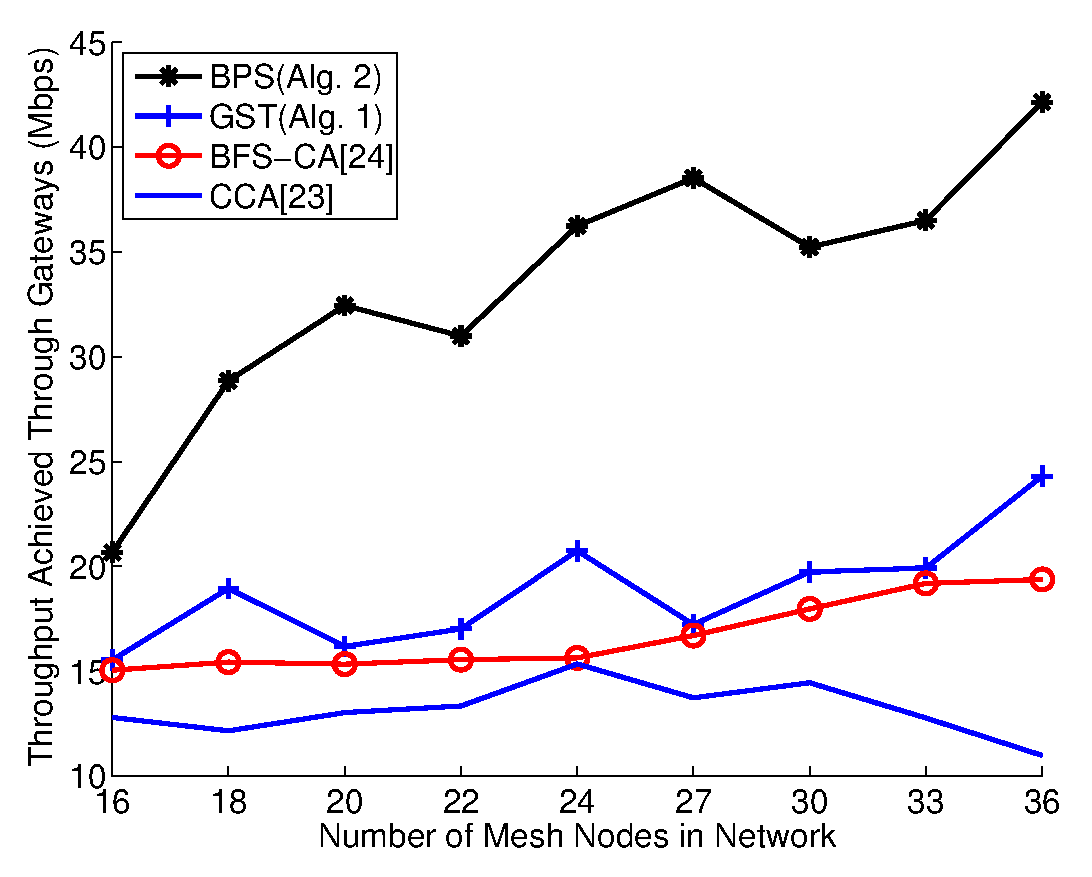
\includegraphics[width=1.6in]{figures/varysize}}
\subfigure[Varying Load, 49-Nodes Regular Grid]{
\label{fig:maxtpt}
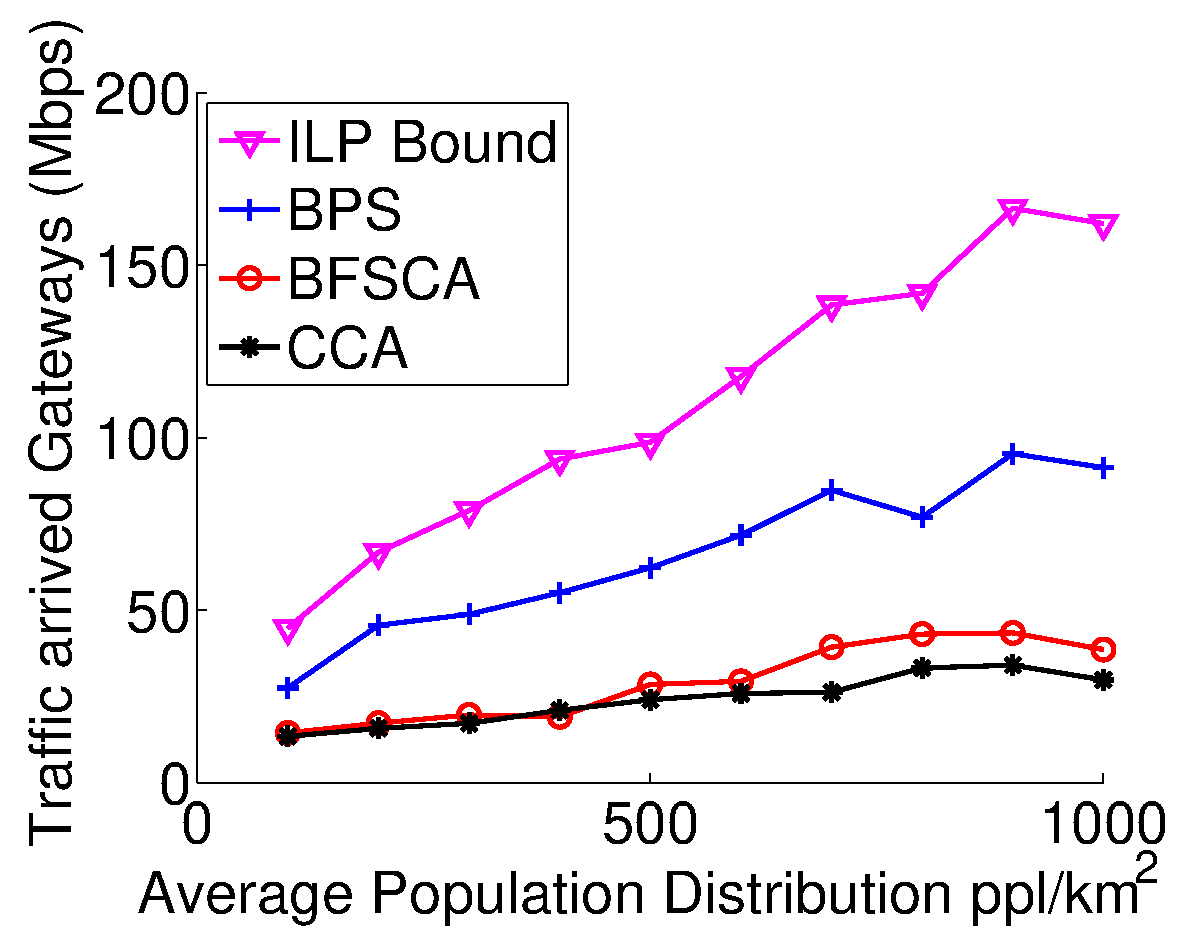
\includegraphics[width=1.6in]{figures/maxtpt.eps}}
\hfill
\caption{Performance in terms of traffic arrived gateway for various offered loads, network sizes, and configurations of WiFi or white space (WS) channels.}
\label{fig:all3figs}
\vspace{-0.1in}
\end{figure}
%\end{figure*}

In Fig.~\ref{fig:varysize}, we observe as the network size increase, the performance
gap among BPS and CCA/BFS-CA goes up. When the network size which represent the size 
of target area, the multiband wireless network has similar communication and interference 
performance with the multi-channel wireless network since all the nodes are located in a 
limited space where could be communicated/interfered by all the bands. As network size 
increase, the connection/interference variation among multiple bands makes the performance 
of multi-channel algorithms stay in low level. The ILP Bound shows what could be expected, 
that an increasing number of gateways/mesh nodes produce an increase in total traffic 
arrived gateways. However, we observe that CCA, BFS-CA algorithms are not able to achieve 
such behavior for various reasons. CCA fails to employ the communication range variation 
and find the most efficient hop connections which increase the average hop count. BFS-CA 
optimizes the first connection hop from the gateway, but fails to deal the whole path 
from the gateway to destination node. Conversely, BPS alleviates the strain on these 
first-hop, bottleneck links, achieving average 76\% of the ILP Bound. The gap of BPS 
to the ILP is part from that the BPS only considers static one path to a gateway node for 
each mesh node, whereas the ILP allows multiple paths to the gateways. For BPS and other 
heuristic algorithms the dynamic assignment could be implemented through updating the 
assignment in a short term.

\begin{table*}
\centering % centering table 
\begin{tabular}{|c|c|c|c|c|c|c|c|c|c|c|c|} % creating 12 columns 
\hline %\hline % inserting double-line 
%Bands     & \multicolumn{3}{c|}{Dallas} & \multicolumn{3}{c|}{Weatherford} & \multicolumn{3}{c|}{Millsap} \\% [0.5ex]
%\hline % inserts single-line 
% Entering 1st row 
 \multirow{2}{*}{Frequency Bands} & \multicolumn{9}{|c|}{Population Distribution $ppl/km^2$} \\
\cline{2-10}
		& 1500 & 1000 & 500 & 300 &  200 & 150 & 100 & 20 & 10 \\ % [0.5ex]
\hline % inserts single-line 
450 MHz &24.37	&25.83  &23.77	&6.05 &12.50  &14.03 & 7.00 & 0.07 & 0.02 \\      
\hline % inserts single-line                                                                                                       
800 MHz &4.40 	&16.49  &4.77	&5.22&5.07 &4.43  & 3.87 & 4.20 & 3.60 \\      
\hline % inserts single-line                                                                                                      
2.4 GHz &15.87 	&34.95  &2.60	&2.03&2.03 &2.77  & 2.07 & 1.60 & 0.80 \\      
\hline % inserts single-line                                                                                                     
5.2 GHz &19.70	&35.46  &1.53	&1.93&1.93 &1.33  & 1.27 & 2.07 & 2.10 \\      
\hline % inserts single-line 
\end{tabular}    
\caption{Activity Level under Population Distribution} % title name of the table 
\label{tab:activitymeasurement}    
\vspace{-0.3in}
\end{table*}    

% Simulation set up
Next, we consider a different form of scalability in our analysis.  Namely,
we increase the average population distribution from 100 to 1,000 per km$^2$, while
maintaining a 49-node regular grid topology. In the simulation set up, we map the
channel capacity to the closest population measurement results. If there are 
measurements has the same distance to the current set up, the lower population 
measurement will be chosen, for instance, we map $400 ppl/km^2$ to $300 ppl/km^2$ 
measurements as shown in Table.~\ref{tab:activitymeasurement}. In Fig.~\ref{fig:maxtpt},
it shows that as the population distribution increases, the ILP and BPS diverge greatly 
from the remaining algorithms. Similar to Fig.~\ref{fig:varysize}, the wireless channel 
capacity around a gateway is quickly saturated if the algorithm is not focused on 
preserving that resource. Another factor of the performance is the channel capacity, 
as population increase the measured channel capacity vary in different bands.
As the population reaches 1,000, the traffic arrived gateways decrease due to the 
channel capacity and the saturation of wireless channel capacity around the gateway
nodes. BPS has an average performance of 60\% of the ILP Bound, on average. CCA and BFS-CA
fails to serve more traffic demand through the jointly WiFi and white space wireless
network. 

\begin{table*}
\centering % centering table 
\begin{tabular}{|l|c|c|c|c|c|c|c|c|c|c|c|} % creating 12 columns 
\hline %\hline % inserting double-line 
Bands/     & WiFi    & WS      & WS \& & WS \& &  WS \& & WS \& & WS \&      &  WS \&      & Multi-WS \& & Multi-WS \& & Multi-WS \& \\% [0.5ex]
Algorithms & Only    & Only    & WiFi  & WiFi  &  WiFi  & WiFi  & Multi-WiFi &  Multi-WiFi & WiFi        & WiFi        & Multi-WiFi  \\
\hline % inserts single-line 
% Entering 1st row 
WS (MHz)   &                                                        & 450,800 & 450 &  800  &  450   & 800               & 450    & 800      & 450,800     & 450,800     & 450,800     \\
\hline
WiFi (GHz) & 2.4, 5 &                                                             & 2.4 &  2.4  &  5   & 5               & 2.4, 5& 2.4, 5        & 2.4             & 5         & 2.4, 5     \\ % [0.5ex]
\hline
\hline % inserts single-line 
CCA~\cite{draves2004routing}                & 22.4   &  13.4  & 13.2    &12.5    & 16.9       & 23.2   &  24.1  &   30.6&  25.2  &       23.9       &   30.4          \\      
\hline % inserts single-line                                                                                                       
BFS-CA~\cite{ramachandran2006interference}  & 26.3   &  15.8  & 14.9    & 19.4   & 22.7       & 28.4   &  38.9  &   33.7&  30.1  &       27.4       &       36.6      \\      
%\hline % inserts single-line                                                                                                      
%GST (Alg. 1)                                                            & 11.6  &   6.6 & 9.3    &   15.1&   15.8        &  14.4  &   16.6   &    14.1  &   18.8            &  15.0           &    25.1         \\      
\hline % inserts single-line                                                                                                     
BPS (Alg. 1)                                & 41.2   & 34.1   &  38.2  & 40.0    & 35.4       & 42.8   & 58.4   &  64.9 &  54.4  &       51.9       &       63.1      \\      
\hline % inserts single-line 
\end{tabular}    
\caption{Throughput achieved through Gateway nodes (Mbps) for various combinations of WiFi and Average Population Distribution = 500 $ppl/km^2$, Network Size = 49 mesh nodes).} % title name of the table 
% NEWClaim fix
\label{tab:2channelcombination}    
\vspace{-0.4in}
\end{table*}    


WhiteMesh networks could be deployed across a vast array of environments, from
rural to urban areas. Each of these areas will have varying amounts of user
demand traffic in proportion to the population densities.  However, 
since a greater number of TV stations exist in urban areas, the available 
white space bands are often inversely related to the population density due to 
the FCC rules~\cite{fccwhitespace}. Also the available channel capacity is 
related to the existing signal activities in the area. To capture these varying
degrees of demand and white space availability we consider three likely scenarios
and one final scenario for comparison purposes: {\it (i)} two WiFi bands (2.4 and
5.8 GHz) channels with two white space channels (450 and 800 MHz), {\it (ii)} 
three channels in two WiFi bands (2.4 and 5.8 GHz) with one white space channel 
(450 MHz), {\it (iii)} Four channels in two WiFi bands (2.4 and 5.8 GHz) without 
any white space channels, and {\it (iv)} four channels in two white space bands 
(450 and 800 MHz) with no WiFi bands (for comparison).

Table~\ref{tab:2channelcombination} describes the achieved traffic arrived gateways 
for various combinations of WiFi and white space bands with a maximum offered load 
of 5 Mbps from 500 $ppl/km^2$ in a regular 49-node grid. We consider the performance 
of BPS in the four aforementioned scenarios of varying white space availability. A 
regular, 49-nodes grid is again used. In the simulation, we keep 4 channels for each
method, such as in the combination of 2.4 GHz and 5 GHz, we put 2 channels in both 
bands. In the triple bands combinations, we set each band has a channel, and put the 
other channel in the highest frequency band. (In 2.4 GHz, 5GHz, 800 MHz combination, 
we put the extra channel other than the 3 channel each band in 5 GHz). 
% Justification
Immediately, we observe that the WiFi-only scenario has greater traffic arrived 
gateways than the white-space-only scenario. This is due to the lack of spatial 
reuse achieved by white spaces. White space has larger communication to shorten 
the hop counts as well as has larger interference reducing the spatial reuse. 
Another reason is that the available channel capacity of 500 $ppl/km^2$ in white 
space bands are worse than WiFi bands. This two reasons make the white space only 
has worse performance no matter what channel assignment methods are applied.
Interestingly, however, the joint use of both white space and WiFi bands has 
significant gains over the single type of band scenarios with the same number of 
channels (40\% greater than WiFi and 56\% over white space, on average). 

In 500 $ppl/km^2$ scenario, 5 GHz channel is cleaner than 450 MHz which makes 
the combination of 2 channels in 5 GHz, 1 channel in 2.4 GHz and 800 MHz has 
better performance than WiFi(2)+WS(2) in some cases.  Obviously, in Table
~\ref{tab:2channelcombination} that with the same number of available bands (2), 
when the combination has similar propagation characters, such as one in WiFi band, 
one in white space band, the combination has clean channels have better performance. 
With similar channel capacity, lower frequency offers more option for connection 
path could output a better channel assignment. If we have one channel in a white 
space band and one channel in a WiFi band, then we could use the advantage of both 
WiFi for spatial reuse and white spaces to reduce the hop count. 



\subsubsection{Effect of Channel Occupancy}

% FIXME include 3 d figure


In Fig.~\ref{fig:actspac}, we show the impacts of channel occupancy through 
the activity level and spacing variation on wireless white space mesh network. 
The activity level defined in~\ref{eq:actlevel} represent the available channel
capacity. The spacing gap is related to the population distribution according to 
the hexagon deployment for access tier network deployment, the more population
distribution, the smaller spacing gap between mesh nodes. In the simulation, we 
assume all the bands have the same activity level and use the 49-nodes regular 
grid with normalized multiple spacing distance gap from 0.2 to 2.1. From the 3-D 
figure, we could see as the activity level increase, the traffic arrived gateways 
decrease due to the deduction of available channel capacity. In the spacing dimension, 
when the nodes have small spacing gap, all the bands could not be applied for 
spacial reuse, the traffic arrived gateways is small. But as the spacing gap 
increase, the spacial reusing is available for high frequency bands, the traffic 
arrived gateways increase. Then, as the spacing gap increase over the high 
frequency communication range, the number of usable channels start to decrease 
according to protocol model, the traffic arrived gateways decrease in the figure.

We further investigate the spacing gap variation under in-field scenario.
The in-field measurement mapping is listed in Table.~\ref{tab:activitymeasurement}. 
We keep the white mesh network as 49-nodes regular grid, assume each mesh 
node has 4 radios in each band. As clarified, a larger spacing gap between mesh 
nodes means less population. We map the largest population distribution in Table
~\ref{tab:activitymeasurement} to represent the spacing as normalized distance 0.2,
and the least population distribution as normalized distance 1.7. 
In a regular grid the spacing distance $D_s$, population distribution $P_d$ and 
mesh node capacity $M_c$ should obey $P_d \cdot \frac{D_s}{2} ^2 \propto M_c$. 
The 9 measured data sets are mapped to generate the matrix sets. Then according 
the data in the matrix we interpolate activity level for each normalized distance 
from 0.2 to 1.7 with gap 0.1. These data sets are put into the heuristic algorithms 
and the results are shown in Fig.~\ref{fig:measurespacing}.

\begin{figure}[t]
\centering
\subfigure[Uniform Activity Level VS. Space Distance]{
\label{fig:actspac}
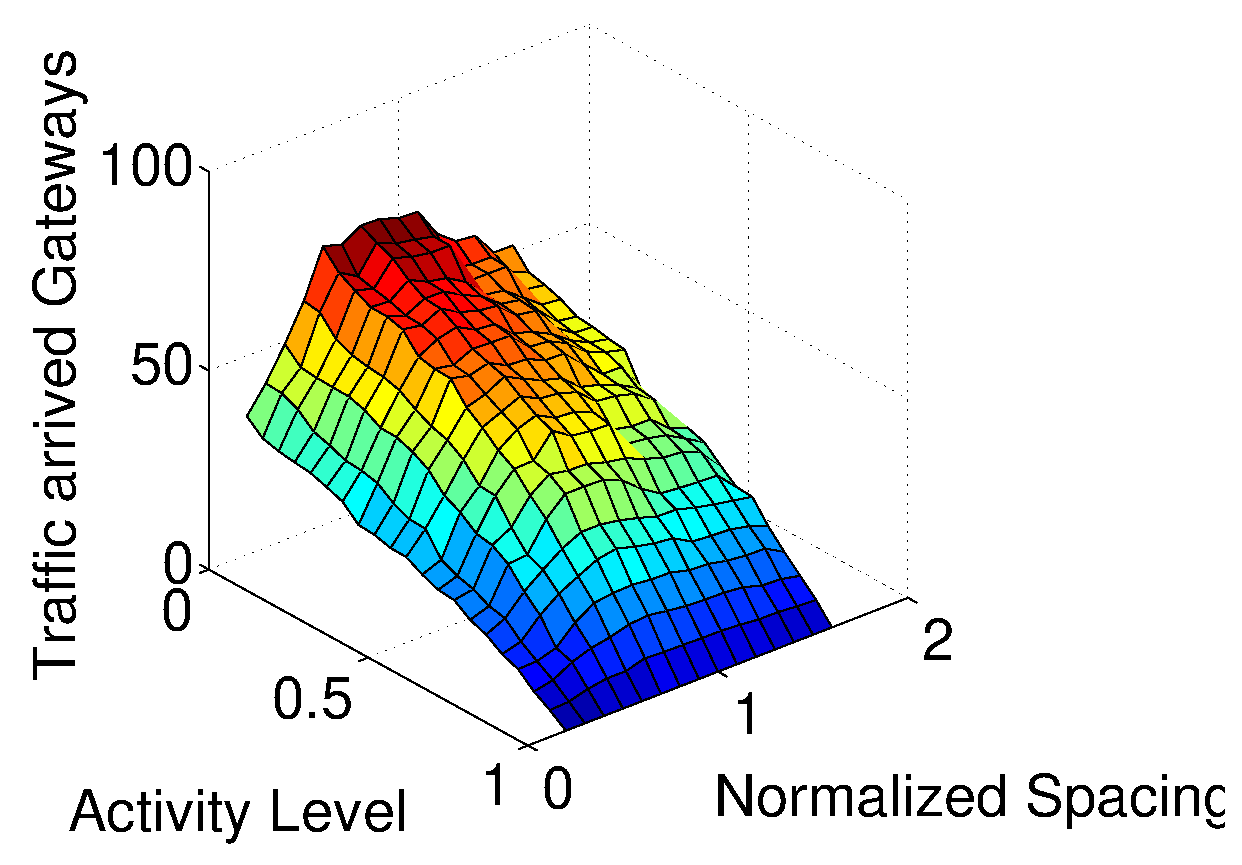
\includegraphics[width=1.6in]{figures/actspac3d}}
\subfigure[Traffic arrived Gateways with Activity Level \& Spacing ]{
\label{fig:measurespacing}
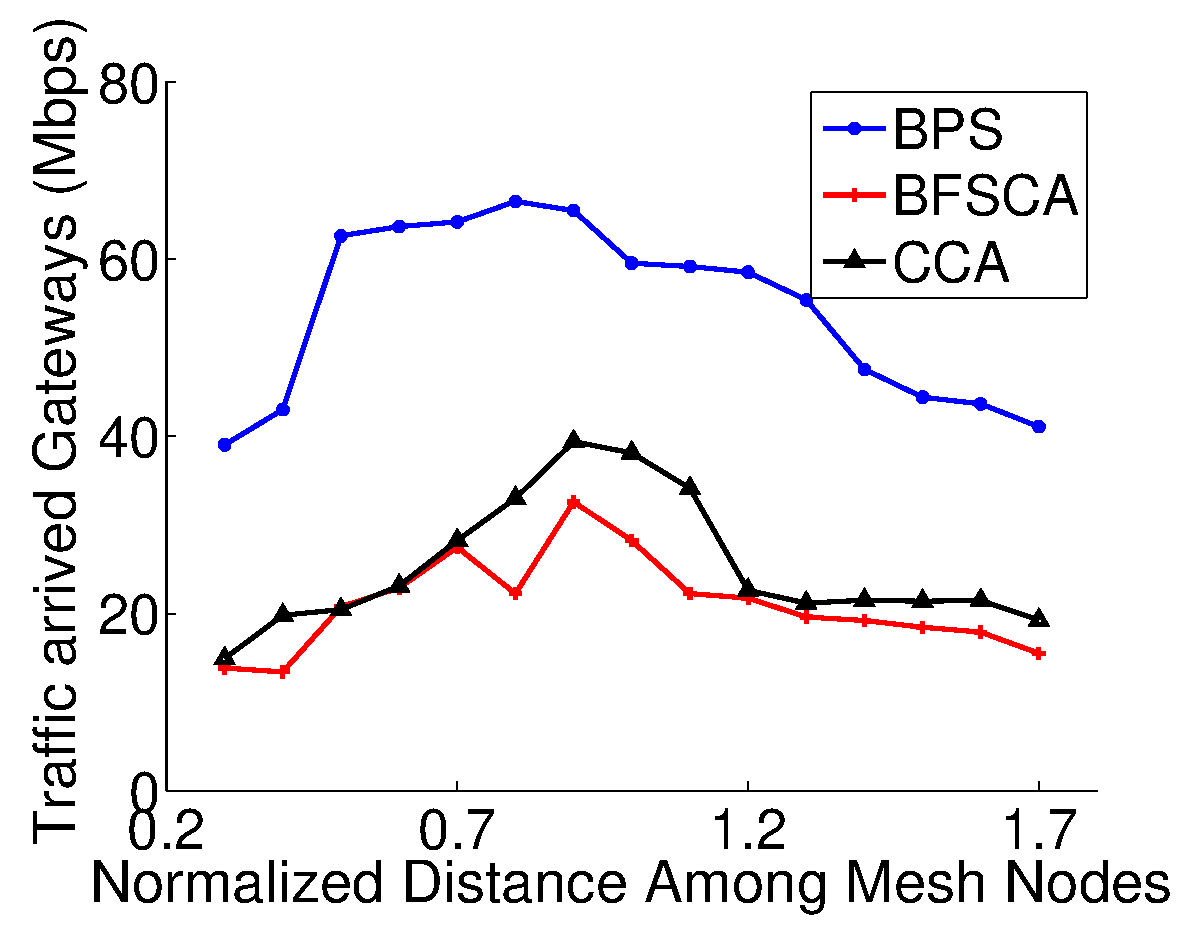
\includegraphics[width=1.6in]{figures/act_spacing}}
\hfill
\caption{}
\label{fig:all3figs}
\vspace{-0.1in}
\end{figure}

In Fig.~\ref{fig:measurespacing}, as the space gap increase, the multiband network 
has better performance through spacial reuse matching the simulation analysis shown 
in Fig.~\ref{fig:actspac}. As the distance increase up to normalized distance 1, one of 
the channel in 5 GHz could not be applied in the network since the distance is larger 
than its communication range under the protocol model, that makes the performance 
decrease quickly. Through this investigation, we can conclude that in sparse area
when the number of mesh nodes is small, lower frequency for the back-hual network 
could have better performance. However, in dense area when the mesh nodes are deployed 
closely, have higher frequency for spacial reuse is better than the low frequency 
white space bands.


Through these analysis, a mixed WiFi and white space wireless network could improve the performance 
in the scenarios as follow: 
{\it (i)} Larger network has more mesh nodes, which 
need more capacity from spacial reuse and flexible path to reduce hop count through
more links. 
{\it (ii)} Rural area whose spacing gap among mesh nodes is larger.
Not only for the number of mesh nodes reducing but also for hop count reducing.
However, as we discussed, the flexible paths and the interference among these
links become more critical at different points in the WhiteMesh topology. 
For the sake of completeness, we need cautious selection of frequency bands
in wireless network deployment.

